%    Documentation for PRU ADC Project
%    Copyright (C) 2016  Gregory Raven
%
%    This program is free software: you can redistribute it and/or modify
%    it under the terms of the GNU General Public License as published by
%    the Free Software Foundation, either version 3 of the License, or
%    (at your option) any later version.
%
%    This program is distributed in the hope that it will be useful,
%    but WITHOUT ANY WARRANTY; without even the implied warranty of
%    MERCHANTABILITY or FITNESS FOR A PARTICULAR PURPOSE.  See the
%    GNU General Public License for more details.
%
%    You should have received a copy of the GNU General Public License
%    along with this program.  If not, see <http://www.gnu.org/licenses/>.

\chapter{Solid State AC Relays}

The BBGW GPIOs are low-current capability with logic voltage of 3.3 volts.  
This solid-state relay board allows the GPIOs to control the irrigation devices:

\url{https://www.amazon.com/gp/product/B00ZZVQR5Q/ref=oh_aui_detailpage_o04_s00?ie=UTF8&psc=1}

\begin{figure}[h]
	\centering
    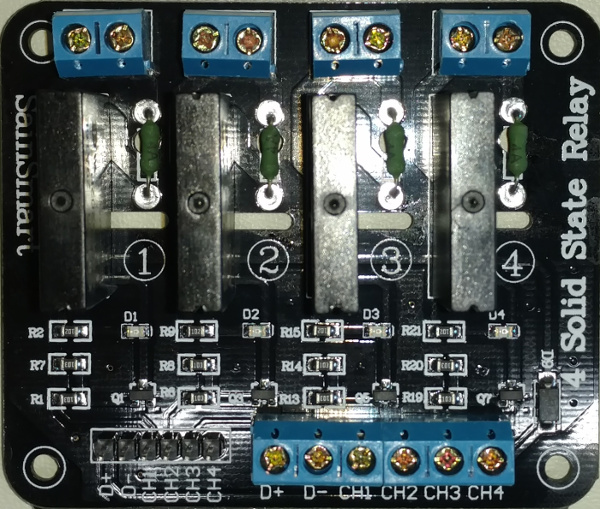
\includegraphics[width=0.5\textwidth]{photos/sainsmart_4relay_board.jpg}
	\centering\bfseries
	\caption{Solid-State Relay Board)}
\end{figure}

Note that in the photo above you can see that the board uses four independent 
solid-state relay modules.  These modules use photo-electric isolation.  This 
should allow excellent protection from voltage transients on the irrigation 
equipment side of the system from damaging the BBGW.  Long-term testing needs 
to be done to see how well this works out.

The individual relay modules require 5 volt logic.  However, there is some 
additional circuitry on the board which appears to allow less than 5 volt 
logic, as long as a 5 volt supply is available.  Unfortunately a circuit 
diagram for this board could not be found.  A ``best guess'' as to the hook-up 
seems to function well.

Viewing the photo of the board above, the screw terminals are labelled:

\begin{verbatim}
D+ D- CH1 CH2 CH3 CH4
\end{verbatim}

The BBGW has 5 volts DC supply available on header pins P9-5 and P9-6 
(VDD\_5V), and also on P9-7 and P9-8 (SYS\_5V).

VDD\_5V is the same as the regulated 5 volt power supply which powers the BBGW 
via the USB connector.  SYS\_5V is switched on immediately after VDD\_5V is 
applied to the board via the USB connector, so functionally it doesn't matter 
which supply is used to power the solid-state-relay input circuitry.

The suggested hook-up is to connect P9-5 to D+, and both of the ground pins 
(P9-1 or P9-2) to D-.  The GPIOs are then connected to CH1, CH2, and CH3 as 
shown in the table:

\begin{longtable}{lll}
\caption{BBGW to Solid-State Relay Interconnect}\\
\toprule
Header Pin & Relay Terminal & Function \\\midrule
P9-1 & D- & Ground \\
P9-2 & D- & Ground \\
P9-5 & D+ & 5 volts \\
P9-14 & CH1 & Pump Motor \\
P9-15 & CH2 & Zone 1 Solenoid \\
P9-16 & CH3 & Zone 2 Solenoid
\end{longtable}
